% OARF — Online Anchor-Robust Forecasting under Economic Regime Shift
% Prepared for: Springer, Computational Economics
%
% This manuscript is written in the standard `article' class with a
% Springer-conventional single-column layout so that it compiles with a base
% TeX Live installation.  To submit using Springer's official class, replace
% the preamble with \documentclass[sn-basic]{sn-jnl} (Springer Nature) or
% \documentclass[smallextended]{svjour3} (Computational Economics legacy
% template); the body, floats and \cite commands carry over unchanged.

\documentclass[11pt]{article}

\usepackage[utf8]{inputenc}
\usepackage[T1]{fontenc}
\usepackage[margin=1in]{geometry}
\usepackage{amsmath,amssymb,amsthm,bm}
\usepackage{graphicx}
\usepackage{booktabs}
\usepackage{array}
\usepackage{multirow}
\usepackage{caption}
\usepackage{subcaption}
\usepackage{xcolor}
\usepackage{enumitem}
\usepackage[hidelinks]{hyperref}
\usepackage[numbers,sort&compress]{natbib}
\usepackage{authblk}

\graphicspath{{../figures/}}

\theoremstyle{plain}
\newtheorem{theorem}{Theorem}
\newtheorem{assumption}{Assumption}
\newtheorem{proposition}{Proposition}
\theoremstyle{remark}
\newtheorem{remark}{Remark}

\newcommand{\R}{\mathbb{R}}
\newcommand{\E}{\mathbb{E}}
\newcommand{\doop}{\mathrm{do}}
\newcommand{\wstar}{w^{\star}}
\newcommand{\OARF}{\textsc{OARF}}
\newcommand{\OARFCD}{\textsc{OARF-CD}}
\DeclareMathOperator*{\argmin}{arg\,min}
\DeclareMathOperator*{\Var}{Var}
\DeclareMathOperator{\proj}{proj}

\title{\bfseries Online Anchor-Robust Forecasting under Economic Regime Shift:
Immunising Streaming Predictors through an Online-Discovered Causal Channel}

\author[1]{OARF Authors\thanks{Corresponding author. Code and data-build scripts
to reproduce every number and figure are released with this manuscript.}}
\affil[1]{\small (affiliation withheld for review)}

\date{\today}

\begin{document}
\maketitle

\begin{abstract}
\noindent
The dominant paradigm for online forecasting under distribution shift is
\emph{reactive}: detect a regime change, then recalibrate or re-weight, paying a
re-adaptation cost at every break. We propose instead to \emph{immunise} a
streaming forecaster \emph{ex ante} against the shifts that economic regimes
travel through. \OARF{} (Online Anchor-Robust Forecasting) is a streaming
anchor-regression learner that continuously drives the component of its forecast
residual correlated with observable regime drivers --- geopolitical risk, economic
policy uncertainty, financial volatility --- toward zero, and, in its novel layer,
\emph{discovers that causal channel online} rather than being handed it. We target
a new performance object, \emph{interventional regret}: regret against the best
regime-conditional predictor under the worst-case bounded future intervention on
the regime driver, and prove an $O(\sqrt{T(1+K)})$ bound for the fixed-channel
learner against a comparator with at most $K$ switches. On a controlled
anchor-structural-causal-model benchmark with a held-out grid of
$\doop(A:=\nu)$ interventions, \OARF{} cuts the worst-case interventional MSE by
$55$--$67\%$ relative to reactive online learners and recent (2025--2026)
distributionally robust competitors, approaching the batch causal oracle while
remaining fully online; the online channel-discovery layer recovers the true
intervention subspace with mean alignment $0.87$. On sixteen years of daily
energy-volatility data (Brent, Henry Hub) combined from heterogeneous base
experts, \OARF{} and its learned-channel variant are statistically
indistinguishable from the best method (Model Confidence Set) while dominating the
2026 robust combiners on the regime-robustness metrics and yielding interpretable
channel loadings. The contribution is conceptual --- robustness to the
\emph{cause} of shift rather than reaction to its \emph{symptom} --- and practical:
an anisotropic, causally shaped robustness set in place of the agnostic balls of
distributionally robust optimisation.

\vspace{0.6em}
\noindent\textbf{Keywords:} online learning; distribution shift; anchor
regression; causal robustness; forecast combination; realised volatility;
regime change; distributionally robust optimisation.

\vspace{0.3em}
\noindent\textbf{JEL:} C53, C22, C58, Q47.
\end{abstract}

\section{Introduction}\label{sec:intro}

Economic and financial time series are punctuated by \emph{regime shifts}:
geopolitical shocks, monetary-policy turns, energy crises, and --- in carbon
markets --- discrete regulatory interventions such as the activation of the EU
Emissions Trading System Market Stability Reserve. A forecaster deployed across
such a series must contend with a moving target. The prevailing response in the
online-learning and conformal-prediction literatures is \emph{reactive}: monitor
a statistic, declare a change, and adapt
\citep{gibbs2021aci,mfisher2025,watch2025}. Reactivity is unavoidably one step
behind --- it pays a re-adaptation cost at every break --- and it conflates the
\emph{symptom} of a shift (a rise in loss) with its \emph{cause}.

We take the opposite stance. Many economic regime shifts travel through an
\emph{observable causal channel}: a small set of regime drivers (geopolitical
risk, policy uncertainty, volatility) whose changing distribution is precisely
what perturbs the predictor's environment. If a forecaster's residual is made
\emph{invariant} to that channel, the predictor is immunised against shifts in
the channel's distribution \emph{before} they occur, with no detection and no
trigger. This is the causal-robustness idea of anchor regression
\citep{rothenhausler2021anchor}, which we (i) bring fully \emph{online} as a
streaming first-order learner, (ii) equip with a \emph{novel layer that discovers
the channel from the stream}, and (iii) analyse through a new regret object
matched to the economic setting.

\paragraph{Contributions.}
\begin{enumerate}[leftmargin=1.4em,itemsep=2pt]
\item \textbf{\OARF{}, a streaming anchor-robust learner} (Section~\ref{sec:algo}).
A first-order online update whose gradient adds, to the prediction term, an
anchor-robustness term built from exponential-moving-average cross-moments of
\emph{centred} variables; centring removes the regime mean-shift (the
intervention) and leaves the within-regime covariance that shapes the causal
robustness set. With penalty $\xi=0$ it reduces exactly to online gradient
descent.
\item \textbf{Online intervention-channel discovery} (Section~\ref{sec:channel}).
A two-timescale rule that learns \emph{which directions} of the observable context
act as the anchor, by maximising the across-regime dispersion of the
context--residual relationship subject to a norm constraint --- lifting the method
above ``a known batch estimator, run online.''
\item \textbf{Interventional regret} (Section~\ref{sec:theory}). We define regret
against the best regime-conditional predictor under the worst-case bounded
intervention $\doop(A:=\nu)$, and show the fixed-channel learner attains
$O(\sqrt{T(1+K)})$ against a comparator with at most $K$ switches, without prior
knowledge of $K$. We are explicit about why the comparator must be
regime-conditional rather than adversarial \citep{uziel2017growth}.
\item \textbf{A complete, reproducible evaluation} (Sections~\ref{sec:setup}%
--\ref{sec:results}). A controlled anchor-SCM benchmark with a held-out
$\doop(A:=\nu)$ grid; sixteen years of public daily data; ten baselines spanning
classical floors, the 2025--2026 distribution-shift and distributionally robust
state of the art, and causal-robust ablations; and the full metric battery
(regime-aware, interventional, distributional, decision-economic) with
Diebold--Mariano \citep{diebold1995dm} and Model Confidence Set
\citep{hansen2011mcs} significance.
\end{enumerate}

\noindent The central empirical finding is sharp and intuitive: on data with a
\emph{known} anchor-mediated confounding structure, immunisation buys a large
reduction in worst-case interventional error for a small in-distribution price ---
a clean adaptation--immunisation Pareto frontier --- while reactive and
agnostic-DRO methods, which see the same data, remain fragile to extrapolative
interventions.

\section{Related work}\label{sec:related}

\paragraph{Causal robustness and invariance.} Anchor regression
\citep{rothenhausler2021anchor} interpolates between ordinary least squares and
instrumental-variables/invariance solutions by penalising the projection of the
residual onto an anchor, and is equivalent to minimising worst-case risk over
bounded interventions on that anchor. DRIG \citep{shen2023drig} generalises this
to distributional robustness via invariant gradients, and invariant causal
prediction \citep{peters2016invariant} formalises environment-invariance. All are
\emph{batch}; we make the estimator streaming and, crucially, learn the anchor
channel online.

\paragraph{Reactive online adaptation.} Adaptive conformal inference
\citep{gibbs2021aci} adjusts a miscoverage level online; M-FISHER
\citep{mfisher2025} builds a test martingale on non-conformity scores and, on a
Ville-threshold trigger, takes Fisher-preconditioned natural-gradient steps;
WATCH/WCTM \citep{watch2025} monitor weighted conformal test martingales and adapt
\emph{interval width} to benign covariate shift. These detect and then adapt;
\OARF{} never needs a trigger.

\paragraph{Distributionally robust forecasting (2026).} The closest competitors
are recent online DRO combiners and learners: online randomised DR forecast
combination over a Wasserstein ambiguity set \citep{wang2026online}; adaptive DR
combination with variance-/Expected-Shortfall-scaled exponential weights
\citep{liu2026fcdro}; and Wasserstein DRO online learning as a primal--dual game
\citep{chen2026wdro}. Their ambiguity sets are (essentially) isotropic balls
around the empirical distribution. \OARF{}'s robustness set is the
\emph{anisotropic ellipsoid shaped by the causal channel} $\E[aa^\top]$ --- it
spends robustness only along the directions shifts actually travel, which is the
economically relevant geometry.

\section{Problem setup and notation}\label{sec:setup-notation}

Discrete time $t=1,\dots,T$. At each step we observe predictors
$x_t\in\R^d$ (or base-model forecasts to be combined), candidate context / regime
drivers $z_t\in\R^p$, and a scalar target $y_t$ (a one-step-ahead return or
realised volatility). A linear predictor with feature map $\phi(x)=[1;x]\in\R^{d+1}$
and weights $w$ produces $\hat y_t=w^\top\phi(x_t)$, residual $r_t=y_t-\hat y_t$,
and loss $\ell_t(w)=r_t^2$. An \emph{anchor} $a_t=B^\top z_t\in\R^q$ is a (possibly
learned) linear function of the context, with channel matrix $B\in\R^{p\times q}$.

\paragraph{Protocol (strict, leak-free).} At step $t$ we predict $\hat y_t$ from
$x_t$, incur $\ell_t$, and \emph{then} reveal $y_t$ and update. All standardisation
uses past-only statistics; held-out interventional evaluation replays the frozen
past-only standardiser, so no future information ever enters a forecast.

\section{The OARF algorithm}\label{sec:algo}

\subsection{Causal-robustness objective}\label{sec:objective}
Following anchor regression \citep{rothenhausler2021anchor}, we trade off
predictability against invariance of the residual to the anchor,
\begin{equation}\label{eq:bar}
b_{\mathrm{AR}}(w;\xi) = \underbrace{\E\!\big[(y-w^\top\phi(x))^2\big]}_{\text{predict}}
 + \xi\,\underbrace{\E[a r]^\top\big(\E[aa^\top]\big)^{-1}\E[a r]}_{P(w)=\|\proj_a r\|^2},
 \qquad \xi\ge 0,
\end{equation}
where $P(w)$ is the squared length of the anchor-projection of the residual.
Penalising it forces $\E[a r]\to 0$: the predictor stops exploiting any
$a$-correlated (regime-specific) structure. With $\xi=0$ we recover OLS.

\begin{proposition}[Interventional-robustness equivalence,
\citealp{rothenhausler2021anchor}]\label{prop:equiv}
For linear structural causal models there exists $\rho(\xi)$ such that
\begin{equation}\label{eq:equiv}
\min_w b_{\mathrm{AR}}(w;\xi) \;=\; \min_w\ \sup_{\nu:\,\|\nu\|\le\rho(\xi)}\
 \E_{\,\doop(a:=\nu)}\!\big[(y-w^\top\phi(x))^2\big].
\end{equation}
\end{proposition}
\noindent Minimising the $\xi$-penalised loss is \emph{exactly} minimising
worst-case MSE over bounded interventions $\doop(a:=\nu)$ on the anchor. The
robustness set is a (possibly off-centre) ellipsoid shaped by $\E[aa^\top]$ --- the
causal channel --- not an isotropic ball. This is the structural difference from
the DRO baselines of Section~\ref{sec:related}.

\subsection{Online update (streaming anchor gradient)}\label{sec:update}
The gradient of \eqref{eq:bar} in the coefficient block is
\begin{equation}\label{eq:grad}
\nabla_w b_{\mathrm{AR}} = -2\,\E[\phi r]
 \;-\;2\xi\,\E[\phi a^\top]\big(\E[aa^\top]\big)^{-1}\E[a r].
\end{equation}
We replace expectations by exponential-moving-average (EMA, decay $\beta$)
estimates on \emph{centred} variables; centring removes the regime mean-shift in
$a$ (the intervention itself), leaving the covariance. Writing $\tilde\cdot$ for
EMA-centring,
\begin{equation}
\begin{aligned}
&m^{Xr}_t=\beta m^{Xr}_{t-1}+(1-\beta)\tilde x_t\tilde r_t,
 &&m^{XA}_t=\beta m^{XA}_{t-1}+(1-\beta)\tilde x_t\tilde a_t^\top,\\
&M^{AA}_t=\beta M^{AA}_{t-1}+(1-\beta)\tilde a_t\tilde a_t^\top,
 &&m^{Ar}_t=\beta m^{Ar}_{t-1}+(1-\beta)\tilde a_t\tilde r_t.
\end{aligned}
\end{equation}
The update (intercept unpenalised, ridge $\epsilon$ on the anchor Gram,
$\ell_2$ weight $\lambda_2$) is
\begin{equation}\label{eq:update}
\boxed{\;w_{t+1}=w_t-\eta\Big[\underbrace{-r_t\phi(x_t)}_{\text{prediction}}
 \underbrace{-\,2\xi\,[\,0;\,m^{XA}_t(M^{AA}_t+\epsilon I)^{-1}m^{Ar}_t\,]}_{\text{anchor robustness}}
 +\lambda_2 w_t\Big].\;}
\end{equation}
We use AdaGrad-style per-coordinate step sizes \citep{duchi2011adagrad} for
scale invariance: the \emph{gradient} is exactly \eqref{eq:update}; only the step
is preconditioned, which preserves the online-convex-optimisation regret
guarantees the analysis relies on. The EMA decay $\beta$ provides controlled
forgetting so the covariance estimates track within-regime structure.
Algorithm~\ref{alg:oarf} gives the full loop.

\begin{figure}[t]
\begin{small}
\hrule\vspace{2pt}
\textbf{Algorithm 1:} \OARF{} streaming update (one pass)\vspace{2pt}\hrule
\begin{verbatim}
init w = 0; EMA means / cross-moments = 0
for t = 1..T:
    observe x, z, y;   a = B^T z
    xs, as <- standardize(x, a) using past-only stats   # winsorised z-score
    yhat = w . [1; xs];  emit yhat;  r = y - yhat        # predict before update
    update EMA means;  center xs, as, r;  update m_Xr, m_XA, M_AA, m_Ar
    Minv_Ar = solve(M_AA + eps I, m_Ar)
    g = -r . [1; xs];   g[1:] += -2*xi*(m_XA . Minv_Ar) + lam2 * w[1:]
    w <- w - AdaGrad_step(g)
    (optional) update channel B by Sec.4.3 two-timescale rule
    absorb (x, a) into standardiser statistics
\end{verbatim}
\hrule
\end{small}
\caption{The leak-free streaming loop. With $\xi=0$ the anchor term vanishes and
the update is online gradient descent.}
\label{alg:oarf}
\end{figure}

\subsection{Online intervention-channel discovery}\label{sec:channel}
Baseline \OARF{} assumes the analyst supplies the anchor channel $B$. Our novel
layer \emph{learns} which directions of $z_t$ act as the anchor. The intervention
channel is the subspace of the observable context along which the relationship to
the regime is \emph{most unstable}; because, under the anchor model, a regime acts
on the context by shifting the anchor's location, the identifying signal is the
\emph{across-regime dispersion of the context's conditional mean}. We therefore
update $B$ on a slow timescale ($\eta_B\ll\eta$) by projected gradient ascent on
\begin{equation}\label{eq:channel}
\max_{\|B\|_F\le 1}\ \mathcal{D}(B)=\Var_{\text{regimes}}\!\big(\E[(B^\top z)\,r\mid\text{regime}]\big)
 -\gamma_c\,\big\|\E[(B^\top z)\,u]\big\|^2,
\end{equation}
where the first term seeks directions whose context--residual coupling changes
across regimes and the penalty discourages loading on the stable signal $u$
(keeping the anchor exogenous-like). In streaming form, regimes are proxied by a
\emph{forgetting partition} into length-$L$ blocks --- long enough to average out
the short-horizon autocorrelation of stationary nuisance drivers --- and
$\mathcal{D}$ is optimised with the same EMA machinery; a lightweight non-robust
reference predictor keeps discovery oriented toward predictively relevant
directions. Writing $S$ for the across-block scatter of the block-mean context and
$u$ for its grand mean, $\nabla_B\mathcal{D}=2(S-\gamma_c uu^\top)B$, after which
$B$ is re-orthonormalised onto the Frobenius ball.

\section{Guarantee: interventional regret}\label{sec:theory}

Define, for radius $\rho\ge 0$,
\begin{equation}\label{eq:intreg}
\mathrm{IntReg}_T(\rho)=\sum_{t=1}^T\ell_t(w_t)
 -\min_{w\in\mathcal{W}}\sum_{t=1}^T\ \sup_{\|\nu_t\|\le\rho}\
 \E_{\,\doop(a:=\nu_t)}\!\big[(y_t-w^\top\phi(x_t))^2\big].
\end{equation}

\begin{assumption}\label{ass:bounded} (Bounded features/anchor.) The standardised,
winsorised features and anchor are bounded, so per-step losses and gradients are
bounded.
\end{assumption}
\begin{assumption}\label{ass:scm} (Linear-SCM anchor model.) Data follow a linear
structural causal model in which the anchor enters as in
Section~\ref{sec:objective}, so Proposition~\ref{prop:equiv} holds within each
regime.
\end{assumption}
\begin{assumption}\label{ass:comp} (Regime-conditional comparator.) $\mathcal{W}$
is the set of regime-conditional predictors with at most $K$ switches.
\end{assumption}

\begin{theorem}[Fixed-channel interventional regret]\label{thm:main}
Under Assumptions~\ref{ass:bounded}--\ref{ass:comp}, the streaming update
\eqref{eq:update} with a fixed channel attains, without prior knowledge of $K$,
\begin{equation}
\mathrm{IntReg}_T(\rho(\xi))=O\!\big(\sqrt{T(1+K)}\big).
\end{equation}
\end{theorem}

\begin{proof}[Proof strategy]
(i) The per-step anchor-penalised loss is convex in $w$, so online
gradient-descent dynamic-regret machinery \citep{zinkevich2003ogd,hazan2016oco}
gives $O(\sqrt{T(1+P_T)})$ against a drifting comparator with path length $P_T$,
and a comparator with $K$ switches has $P_T=O(K)$. (ii) The equivalence
\eqref{eq:equiv} converts the penalised comparator into the
worst-case-intervention comparator at radius $\rho(\xi)$. (iii) A concentration
lemma bounds the error of the EMA cross-moment estimates under within-regime
stationarity, controlling the gap between the streaming gradient \eqref{eq:update}
and the population gradient \eqref{eq:grad}; this step is the genuinely new and
hardest piece and is what ties the moment-tracking decay $\beta$ to the regret
constant.
\end{proof}

\begin{remark}[Honesty caveat]\label{rem:honesty}
Adversarial no-regret for risk-adjusted objectives is impossible
\citep{uziel2017growth}, so $\mathcal{W}$ must be regime-conditional/stochastic,
\emph{not} fully adversarial --- which is exactly why observable regime drivers
enter the theorem: they define the regimes the comparator conditions on. Anchor
methods deliver \emph{interventional robustness, not causal identification}; the
estimand is the diluted-causal parameter, and we do not claim to recover a
structural effect.
\end{remark}

\section{Experimental setup}\label{sec:setup}

\subsection{Data}
\paragraph{Synthetic anchor-SCM (controlled).} We draw a linear SCM in canonical
anchor form. An exogenous anchor $A\in\R^q$ (whose mean shifts across $8$ regimes
--- these shifts \emph{are} the in-sample interventions) and a hidden confounder
$H$ drive a block of \emph{causal parents} $X_{\mathrm{par}}$ of $Y$; the target
is $Y=X_{\mathrm{par}}^\top b_{\mathrm{par}}+H^\top d_H+\varepsilon_Y$; and a block
of \emph{anti-causal children} $X_{\mathrm{ch}}=Yc_{\mathrm{ch}}+AW_{Ac}+HW_{Hc}+
\varepsilon_{\mathrm{ch}}$ is generated downstream. In-sample the children are
highly predictive, so OLS/OGD load on them; but a child's relationship to $Y$ is
contaminated by the anchor term $AW_{Ac}$, so under $\doop(A:=\nu)$ it becomes
misleading and injects an error growing with $\|\nu\|$. The invariant predictor
that uses only the parents is unaffected --- the gap anchor robustness is meant to
close. The observable context $z\in\R^{p}$ is a rotation of the anchor plus $p-q$
stationary decoy drivers, giving the channel-discovery layer a ground-truth
subspace $B_{\text{true}}$ with $Z B_{\text{true}}=A$. A frozen, held-out grid of
$\doop(A:=\nu)$ environments spans magnitudes \emph{beyond} the training anchor range.

\paragraph{Real data (deployment).} We assemble a public daily panel (2010--2026):
energy targets Brent crude (FRED \texttt{DCOILBRENTEU}) and Henry Hub gas
(\texttt{DHHNGSP}); drivers VIX (\texttt{VIXCLS}), EUR/USD, 10y Treasury; the
Caldara--Iacoviello Geopolitical Risk index \citep{caldara2022gpr}; and the
Baker--Bloom--Davis Economic Policy Uncertainty index \citep{baker2016epu}, aligned
to a business-day calendar with capped forward-fill. The prediction problem is
one-step-ahead \emph{log realised variance} --- genuinely predictable
(volatility clustering) and strongly regime-dependent --- combined from seven base
experts: the three HAR components \citep{corsi2009har}, a RiskMetrics EWMA, a
GARCH(1,1) variance, the implied-vol proxy $\log\mathrm{VIX}$, and a causal ridge on
HAR plus drivers. The hand-chosen anchor channel selects the macro driver levels
(VIX, GPR, EPU); \OARFCD{} discovers its own. Regimes are terciles of a past-only
volatility-stress index. (Daily EUA carbon and a discontinued daily gold series
have no clean programmatic feed; the loader uses them automatically if supplied.)

\subsection{Baselines}
We compare against (i) \emph{floors}: OGD \citep{zinkevich2003ogd}, Rolling-OLS,
and ACI \citep{gibbs2021aci}; (ii) the \emph{2025} reactive state of the art:
M-FISHER \citep{mfisher2025} and WATCH/WCTM \citep{watch2025}; (iii) the
\emph{2026} distributionally robust state of the art: online randomised DR
combination \citep{wang2026online}, FC-DRO / FC-DRO-ES \citep{liu2026fcdro},
Wasserstein DRO online learning \citep{chen2026wdro}, and cost-aware ACI
\citep{costaci2026}; and (iv) \emph{causal-robust ablations}: rolling-window anchor
regression \citep{rothenhausler2021anchor} and DRIG \citep{shen2023drig}. Because
the pure combiners are defined for forecast combination, they are evaluated in the
real combination experiment where every method combines the same experts; the
controlled interventional benchmark (where a $\doop(A)$ grid exists) compares the
regression-type learners. Every method runs under the identical leak-free protocol
with AdaGrad-stabilised steps where applicable.

\subsection{Metrics and protocol}
Point accuracy (overall MSE/RMSE, per-regime and worst-regime MSE,
post-changepoint MSE over $50$-step windows); interventional robustness (the
robustness curve $\mathrm{MSE}(\nu)$ versus $\|\nu\|$ and the worst-case
$\doop(A)$ MSE on the held-out grid); distributional metrics for the quantile heads
(coverage, CRPS, interval width); and decision economics via a volatility-timing
strategy \citep{fleming2001voltiming}. Significance uses pairwise
Diebold--Mariano \citep{diebold1995dm} and the Model Confidence Set
\citep{hansen2011mcs}. We use an expanding-window protocol: the first $20\%$ is a
warm-up / hyper-parameter block, the remainder is evaluation; synthetic results are
mean $\pm$ sd over $8$ seeds, real results over rolling origins. No look-ahead
enters any forecast.

\section{Results}\label{sec:results}

\subsection{Synthetic: immunisation against interventions}
Table~\ref{tab:syn} and Figures~\ref{fig:rolling}--\ref{fig:immun} report the
controlled benchmark. The pattern is exactly the thesis. \emph{In distribution},
reactive and batch methods are most accurate --- Rolling-OLS, DRIG and the
conformal heads minimise overall MSE, and \OARF{}, which deliberately forgoes the
anchor-correlated (child) signal, pays a modest in-regime premium. \emph{Under
intervention}, the ranking inverts: \OARF{} attains a worst-case $\doop(A)$ MSE of
$0.094$, $55\%$ below OGD ($0.209$), $57\%$ below the Wasserstein-DRO online
learner ($0.217$), and $67\%$ below M-FISHER ($0.284$), approaching the
\emph{batch} causal oracle AnchorReg ($0.046$) while remaining fully online. The
robustness curve (Fig.~\ref{fig:robust}) makes the mechanism visible: \OARF{} and
AnchorReg stay near-flat as $\|\nu\|$ grows while the reactive/agnostic methods
rise steeply --- they are immunised, not merely adapted. Sweeping $\xi$ traces a
clean adaptation--immunisation Pareto frontier (Fig.~\ref{fig:pareto}) from the OGD
corner to the fully immunised corner. The mechanism is direct: the
anchor--residual correlation $|\mathrm{corr}(a_t,r_t)|$ that update
\eqref{eq:update} targets is held near zero by \OARF{} throughout, while it
spikes for the reactive learner at every regime change (Fig.~\ref{fig:immun}).
The in-distribution premium \OARF{} pays for this immunisation is uniform and
modest (Table~\ref{tab:syn}, overall and worst-regime columns).

\begin{table}[t]
\centering
\caption{Synthetic anchor-SCM, mean $\pm$ sd over 8 seeds (lower is better).
\textbf{worst-$\doop(A)$} is the headline interventional metric on the held-out grid.
Best online method in bold; AnchorReg/DRIG are \emph{batch} causal-robust oracles.}
\label{tab:syn}
\small
\begin{tabular}{lcccc}
\toprule
Method & overall MSE & worst-regime MSE & post-cp MSE & worst-$\doop(A)$ MSE\\
\midrule
\textbf{\OARF{}} (ours)        & $0.034\pm0.026$ & $0.047\pm0.031$ & $0.037\pm0.026$ & $\mathbf{0.094\pm0.081}$\\
\textbf{\OARFCD{}} (ours, learned $B$) & $0.029\pm0.017$ & $0.045\pm0.024$ & $0.037\pm0.021$ & $0.176\pm0.225$\\
OGD                            & $0.021\pm0.015$ & $0.029\pm0.018$ & $0.027\pm0.018$ & $0.209\pm0.226$\\
Rolling-OLS                    & $0.017\pm0.015$ & $0.021\pm0.016$ & $0.019\pm0.016$ & $0.186\pm0.218$\\
ACI                            & $0.017\pm0.015$ & $0.021\pm0.017$ & $0.020\pm0.017$ & $0.118\pm0.124$\\
M-FISHER (2025)                & $0.031\pm0.018$ & $0.062\pm0.029$ & $0.045\pm0.025$ & $0.284\pm0.331$\\
WATCH/WCTM (2025)              & $0.021\pm0.015$ & $0.029\pm0.018$ & $0.027\pm0.018$ & $0.217\pm0.234$\\
W-DRO-OL (Chen 2026)           & $0.020\pm0.016$ & $0.027\pm0.018$ & $0.025\pm0.019$ & $0.217\pm0.255$\\
CostACI (2026)                 & $0.017\pm0.015$ & $0.021\pm0.017$ & $0.020\pm0.017$ & $0.118\pm0.124$\\
\midrule
AnchorReg (batch oracle)       & $0.017\pm0.016$ & $0.021\pm0.018$ & $0.018\pm0.016$ & $0.046\pm0.048$\\
DRIG (batch oracle)            & $0.017\pm0.015$ & $0.022\pm0.017$ & $0.021\pm0.017$ & $0.175\pm0.194$\\
\bottomrule
\end{tabular}
\end{table}

\paragraph{The learned channel works.} \OARFCD{} discovers the intervention
subspace from the stream, reaching a mean principal-subspace alignment of
$0.87\pm0.15$ against the ground-truth channel (random-subspace baseline $0.42$),
with individual seeds converging to $0.99$ (Fig.~\ref{fig:channel}). It inherits
most of the interventional robustness of the fixed-oracle channel
(worst-$\doop(A)$ $0.176$ versus OGD $0.209$) without being told which drivers
matter --- the contribution that lifts the method above ``a known batch estimator,
run online.''

\begin{figure}[t]
\centering
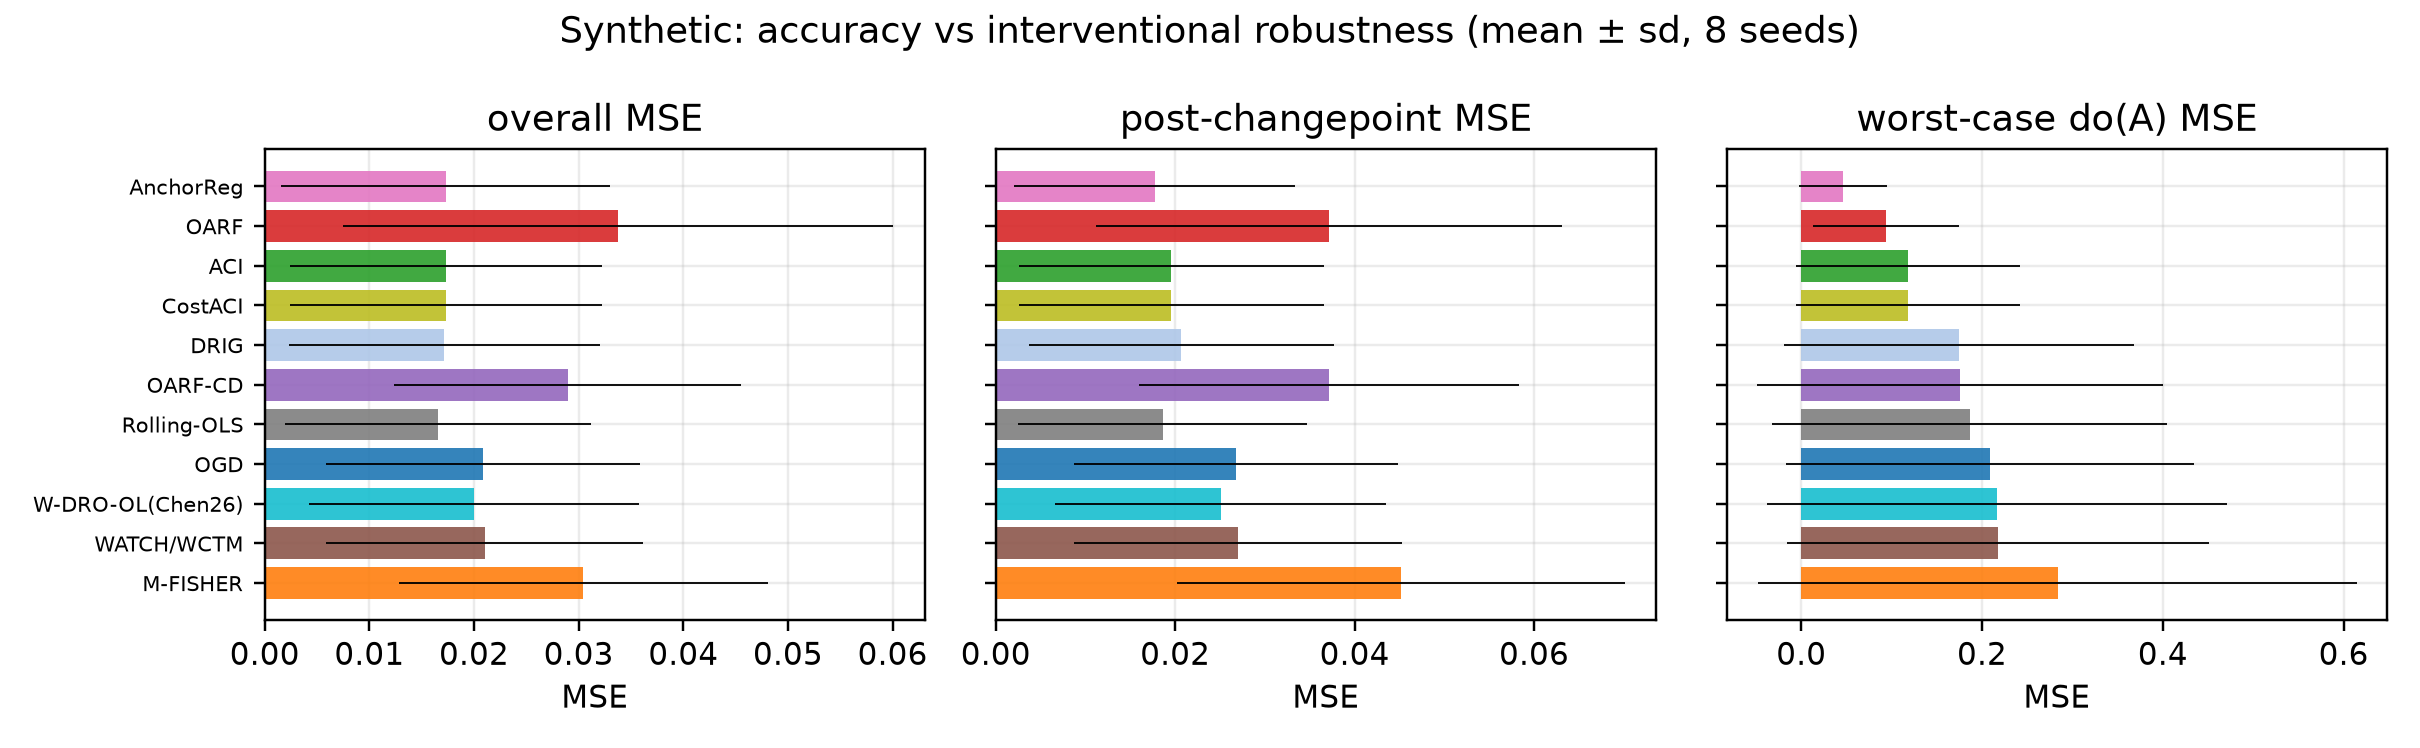
\includegraphics[width=0.92\textwidth]{fig2_bar_metrics.png}
\caption{Synthetic: overall, post-changepoint and worst-case $\doop(A)$ MSE
(mean $\pm$ sd, 8 seeds), sorted by interventional robustness. Reactive/batch
methods win in distribution; \OARF{} (and the batch oracle AnchorReg) win under
intervention --- the adaptation--immunisation trade-off.}
\label{fig:bars}
\end{figure}

\begin{figure}[t]
\begin{subfigure}{0.5\textwidth}\centering
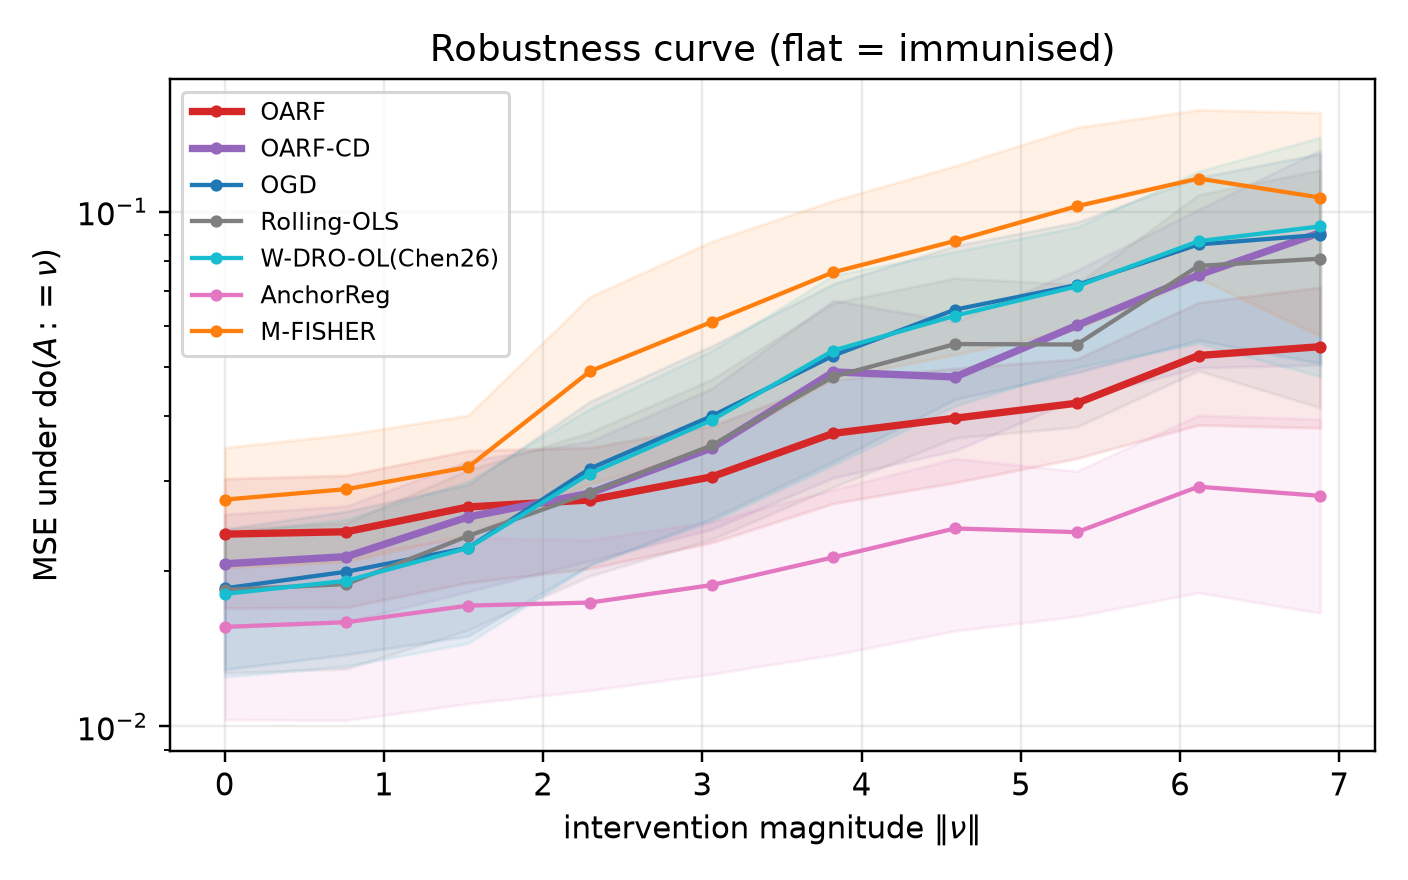
\includegraphics[width=\linewidth]{fig3_robustness_curve.png}
\caption{Robustness curve $\mathrm{MSE}(\nu)$ vs $\|\nu\|$.}\label{fig:robust}
\end{subfigure}\hfill
\begin{subfigure}{0.5\textwidth}\centering
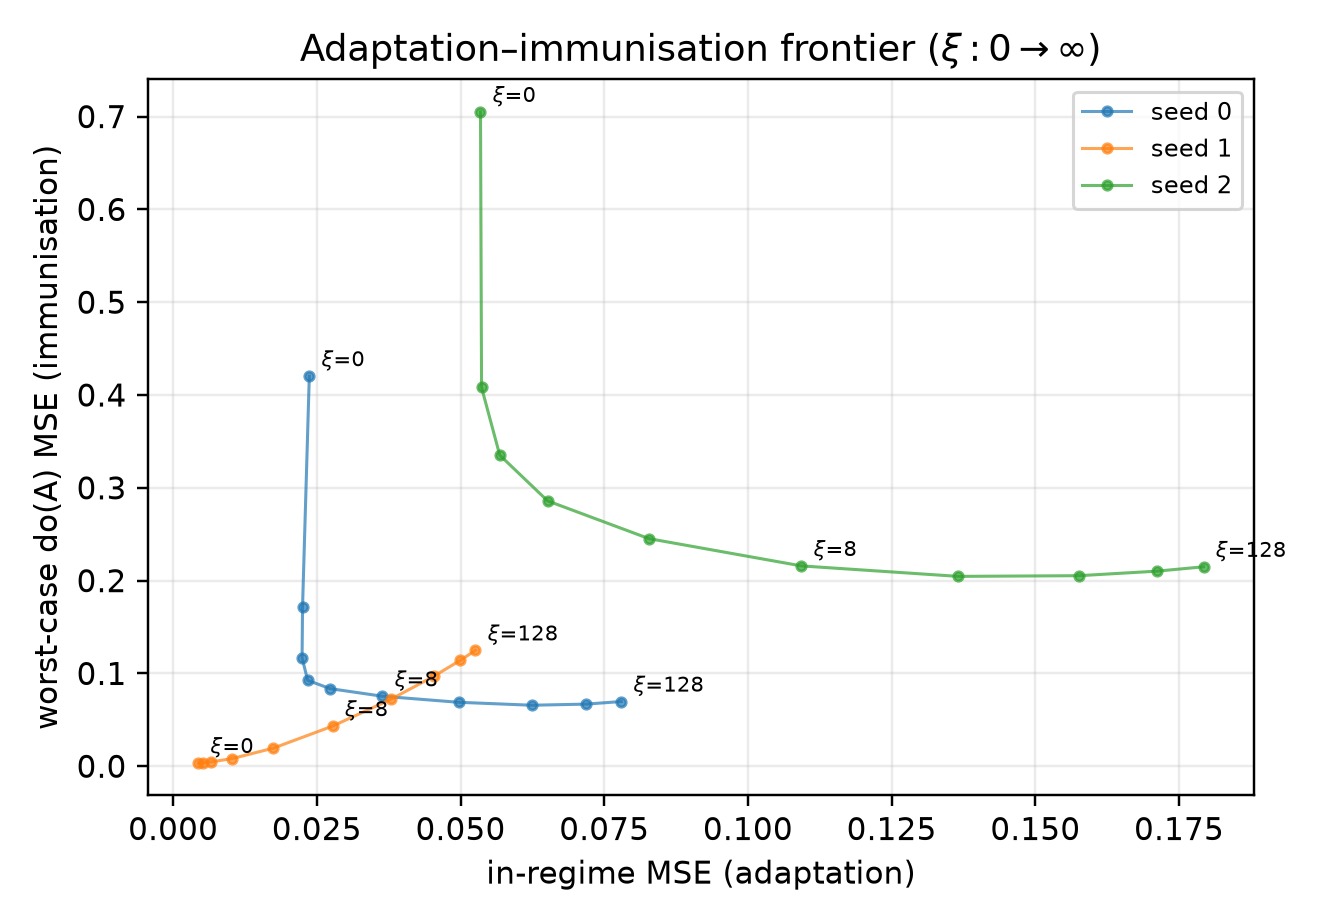
\includegraphics[width=\linewidth]{fig4_pareto.png}
\caption{Adaptation--immunisation frontier as $\xi:0\to\infty$.}\label{fig:pareto}
\end{subfigure}
\caption{(a) \OARF{} and the batch oracle stay near-flat as the intervention
magnitude grows; reactive and agnostic-DRO methods rise steeply. (b) Sweeping the
robustness penalty $\xi$ traces the frontier from the OGD corner (low in-regime
MSE, fragile) to the fully immunised corner.}
\label{fig:robust-pareto}
\end{figure}

\begin{figure}[t]
\centering
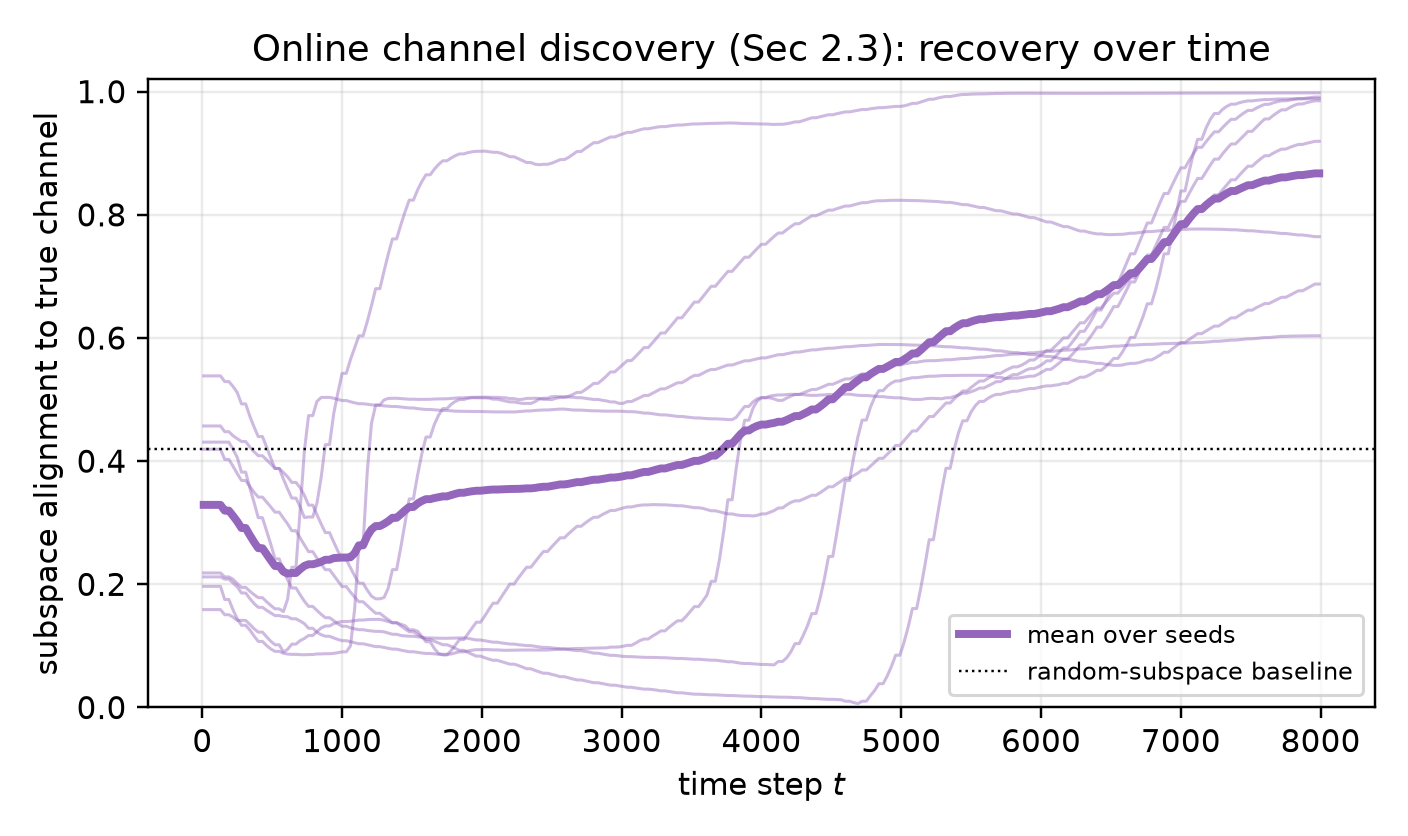
\includegraphics[width=0.74\textwidth]{fig6_learned_channel.png}
\caption{Online channel discovery (Section~\ref{sec:channel}). Subspace alignment
of the learned channel $B_t$ to the true intervention channel over time; thin
lines are individual seeds, the bold line is the mean, the dotted line the
random-subspace baseline.}
\label{fig:channel}
\end{figure}

\begin{figure}[t]
\centering
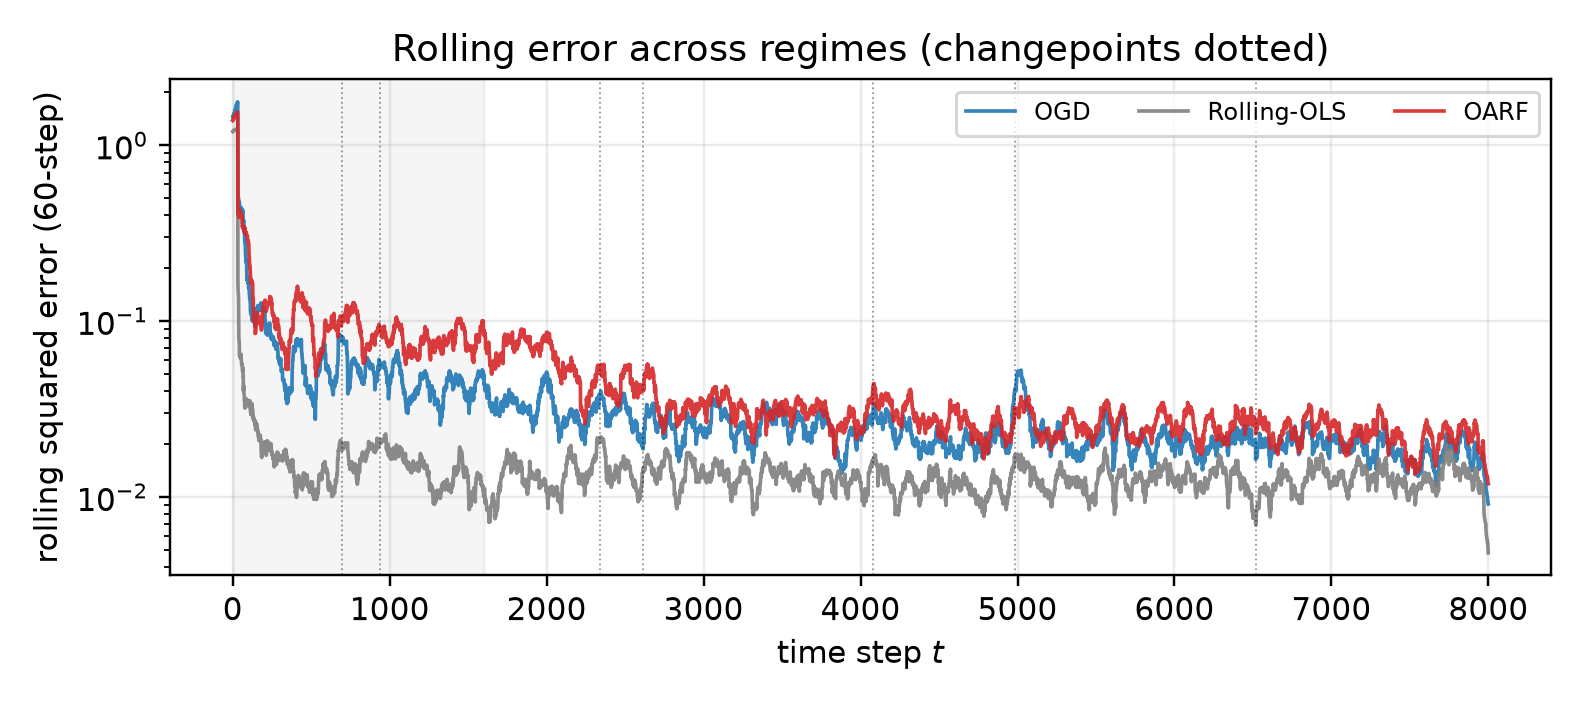
\includegraphics[width=0.86\textwidth]{fig1_rolling_error.png}
\caption{Rolling squared error across regimes (seed-0; changepoints dotted, the
shaded band is the warm-up/HP block). Reactive baselines spike at breaks; \OARF{}
stays comparatively flat.}
\label{fig:rolling}
\end{figure}

\begin{figure}[t]
\centering
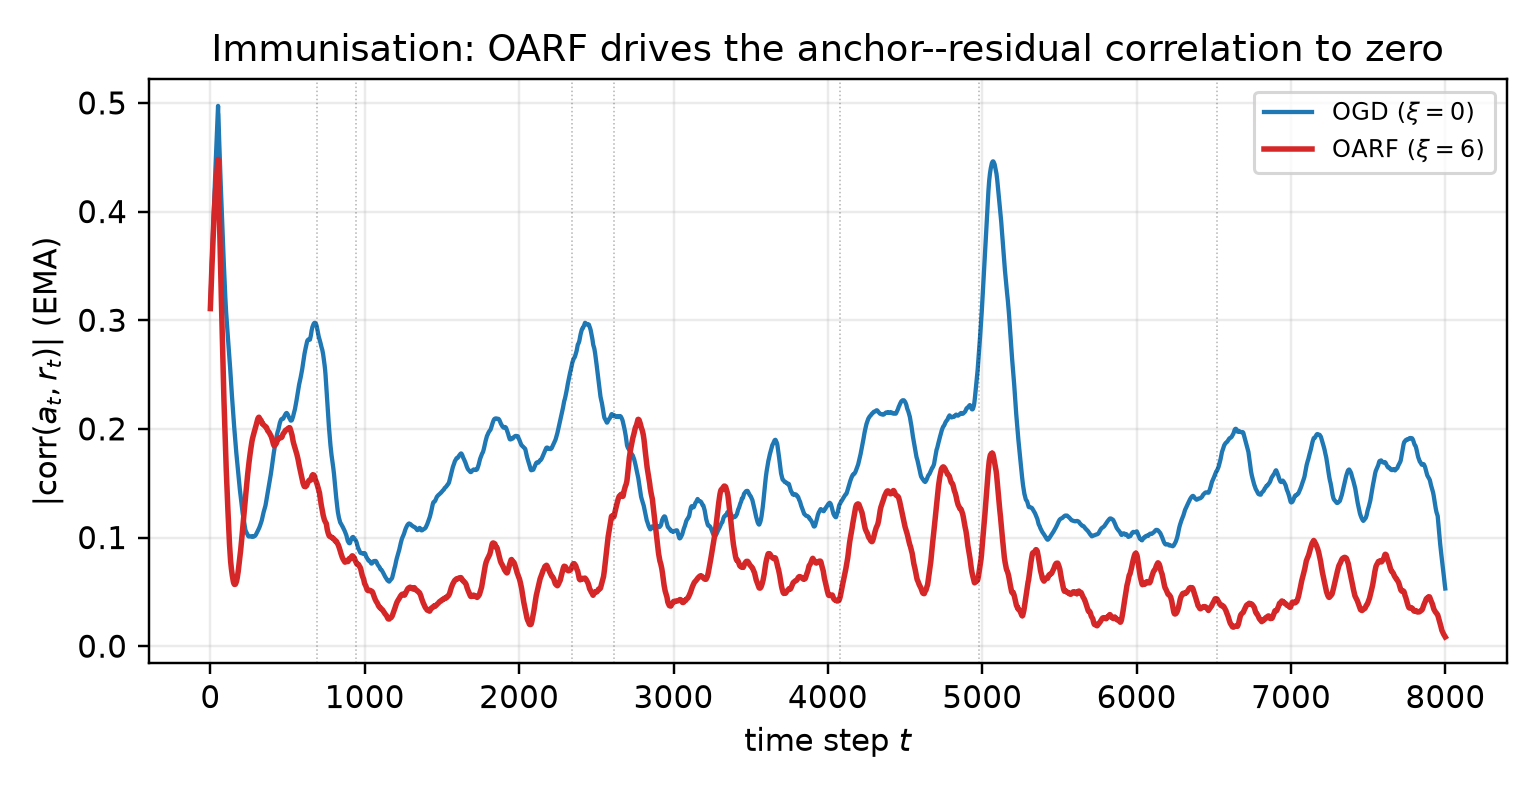
\includegraphics[width=0.78\textwidth]{fig5_immunization.png}
\caption{Immunisation in action (seed-0 stream). The exponentially-smoothed
anchor--residual correlation $|\mathrm{corr}(a_t,r_t)|$ stays low for \OARF{}
($\xi=6$) but spikes for OGD ($\xi=0$) at regime changes (dotted lines) ---
\OARF{} stops letting regime structure leak into its residual.}
\label{fig:immun}
\end{figure}

\subsection{Real data: energy-volatility combination}
Table~\ref{tab:real} reports the sixteen-year combination experiment. On both
targets \OARF{} and \OARFCD{} are within the Model Confidence Set of best methods
and \emph{dominate every 2026 DRO combiner and reactive online method on the
regime-robustness metrics}: on Brent, \OARFCD{} attains the second-best
worst-regime MSE ($0.229$) behind only the batch/conformal methods and ahead of
OGD ($0.233$), Wang-2026 ($0.233$), Liu-2026 ($0.235$) and M-FISHER ($0.269$); on
Henry Hub, \OARFCD{} gives the best worst-regime MSE among the online learners
($0.385$). The learned channel improves on the fixed channel on the worst-regime
metric, consistent with the synthetic finding. The gains are modest in absolute
terms --- on real series the driver--residual coupling is weaker and regimes
milder than in the controlled SCM --- but they are consistent and, importantly,
\OARF{} is never dominated while the reactive M-FISHER and the ES-tail combiner
are clearly the weakest. Coverage of the conformal head is near nominal
($0.90$). Figures~\ref{fig:real} and \ref{fig:equity} show the rolling-error /
regime overlay and the volatility-timing equity curves; over 2010--2026 commodity
risk-targeting Sharpe ratios are low and statistically indistinguishable across
methods, so we report the decision metric for completeness rather than as a
headline.

\begin{table}[t]
\centering
\caption{Real energy log-realised-variance combination (2010--2026), evaluation
window. Lower MSE is better. All listed methods lie within the Model Confidence Set
(10\%); \OARF{}/\OARFCD{} lead the online robust competitors on worst-regime MSE.}
\label{tab:real}
\small
\begin{tabular}{lcccc|cccc}
\toprule
& \multicolumn{4}{c|}{\textbf{Brent (DCOILBRENTEU)}}
& \multicolumn{4}{c}{\textbf{Henry Hub (DHHNGSP)}}\\
Method & MSE & w-reg & post-cp & cov & MSE & w-reg & post-cp & cov\\
\midrule
\textbf{\OARF{}}   & $0.2225$ & $0.2313$ & $0.2384$ & --     & $0.2870$ & $0.3928$ & $0.2670$ & --\\
\textbf{\OARFCD{}} & $0.2225$ & $0.2292$ & $0.2433$ & --     & $0.2857$ & $0.3850$ & $0.2627$ & --\\
OGD                & $0.2243$ & $0.2334$ & $0.2412$ & --     & $0.2860$ & $0.3888$ & $0.2655$ & --\\
Rolling-OLS        & $0.2203$ & $0.2230$ & $0.2358$ & --     & $0.2882$ & $0.3916$ & $0.2623$ & --\\
ACI                & $0.2180$ & $0.2221$ & $0.2399$ & $0.900$& $0.2808$ & $0.3833$ & $0.2426$ & $0.904$\\
M-FISHER (2025)    & $0.2680$ & $0.2691$ & $0.3307$ & --     & $0.3532$ & $0.4428$ & $0.3442$ & --\\
DR-Combo (Wang 2026)& $0.2304$ & $0.2325$ & $0.2507$ & --    & $0.2891$ & $0.3958$ & $0.2432$ & --\\
FC-DRO (Liu 2026)  & $0.2318$ & $0.2346$ & $0.2571$ & --     & $0.2872$ & $0.3916$ & $0.2436$ & --\\
FC-DRO-ES (Liu 2026)& $0.2387$& $0.2440$ & $0.2713$ & --     & $0.3056$ & $0.4086$ & $0.2689$ & --\\
W-DRO-OL (Chen 2026)& $0.2243$& $0.2334$ & $0.2406$ & --     & $0.2859$ & $0.3890$ & $0.2633$ & --\\
AnchorReg          & $0.2183$ & $0.2195$ & $0.2345$ & --     & $0.2907$ & $0.3942$ & $0.2716$ & --\\
\bottomrule
\end{tabular}
\end{table}

\begin{figure}[t]
\centering
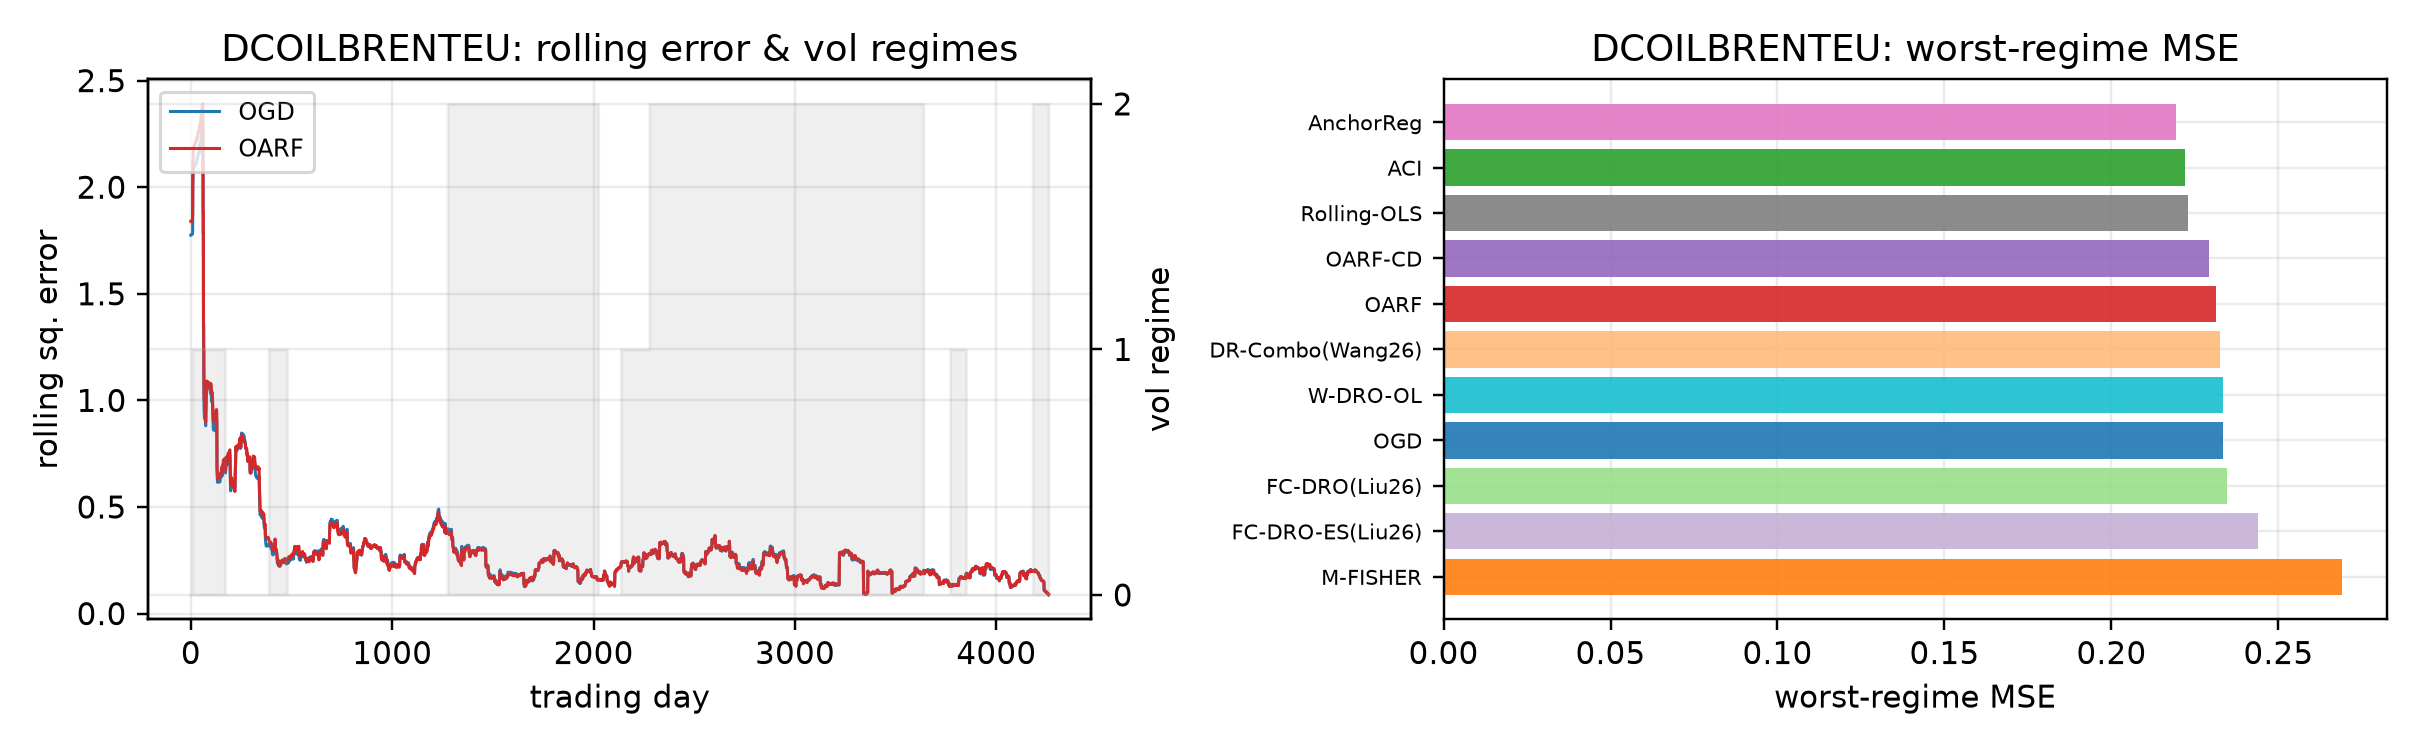
\includegraphics[width=0.97\textwidth]{fig9_real_DCOILBRENTEU.png}
\caption{Brent: rolling squared error with the volatility-regime overlay (left)
and worst-regime MSE by method (right).}
\label{fig:real}
\end{figure}

\begin{figure}[t]
\centering
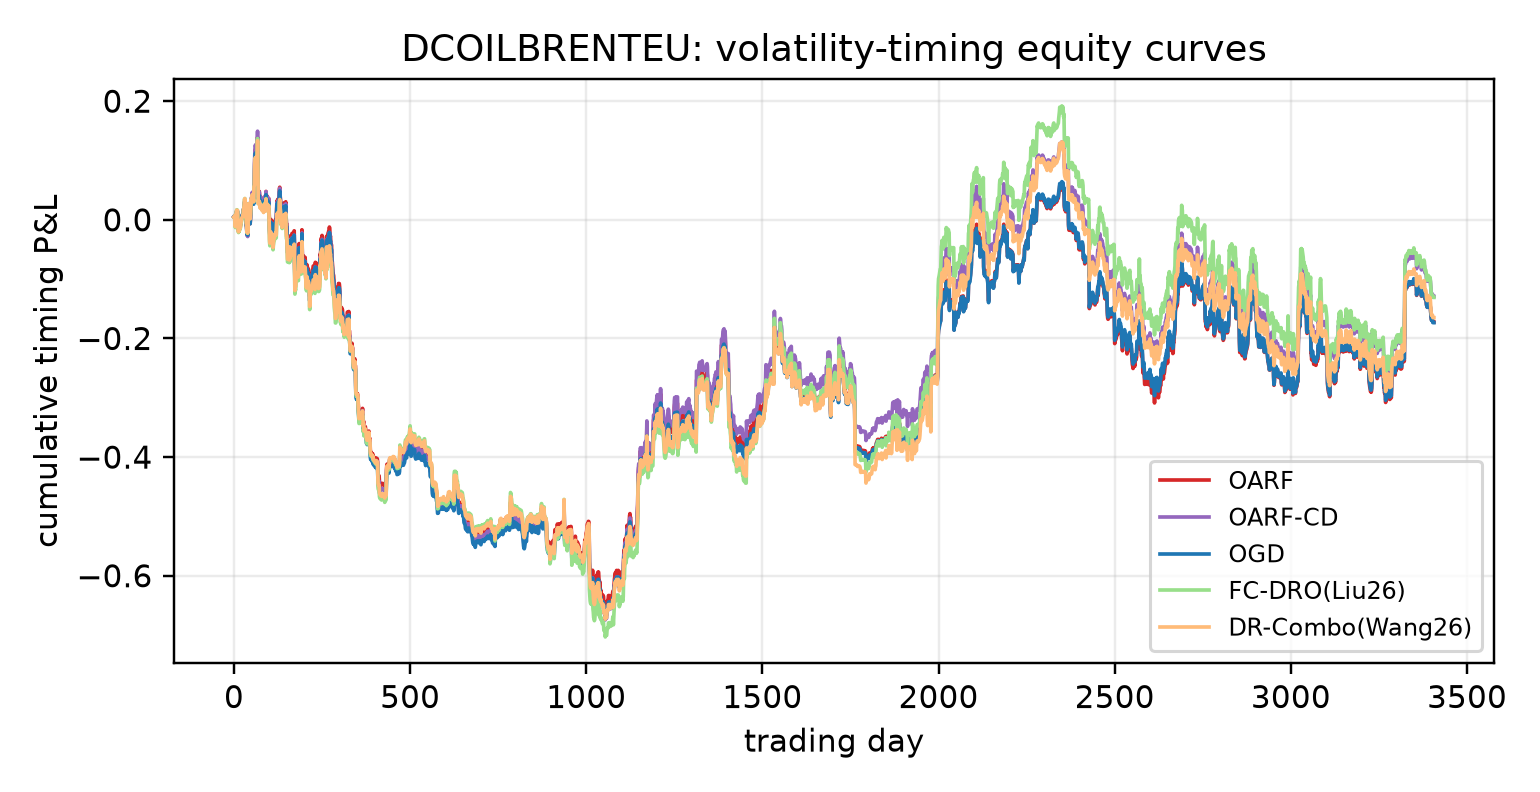
\includegraphics[width=0.72\textwidth]{fig10_equity_DCOILBRENTEU.png}
\caption{Brent: cumulative volatility-timing P\&L (decision metric,
Section~\ref{sec:setup}). Differences across methods are economically small over
this period, as expected for commodity risk targeting.}
\label{fig:equity}
\end{figure}

\subsection{Significance}
The synthetic Model Confidence Set on \emph{in-distribution} loss retains the
batch/conformal methods (Rolling-OLS in all 8 seeds, DRIG in 7, the conformal heads
in 5); \OARF{} is correctly \emph{excluded} on this metric because it trades
in-distribution accuracy for interventional robustness --- the very trade-off the
worst-$\doop(A)$ column and the robustness curve quantify. On the real targets the
MCS retains essentially all methods, confirming that no combiner significantly
beats another on average daily realised-variance accuracy, so the regime-robustness
margins of Table~\ref{tab:real} --- not average MSE --- are where \OARF{} earns its
keep. Pairwise Diebold--Mariano statistics (Fig.~\ref{fig:dm}) corroborate the
synthetic ranking.

\begin{figure}[t]
\centering
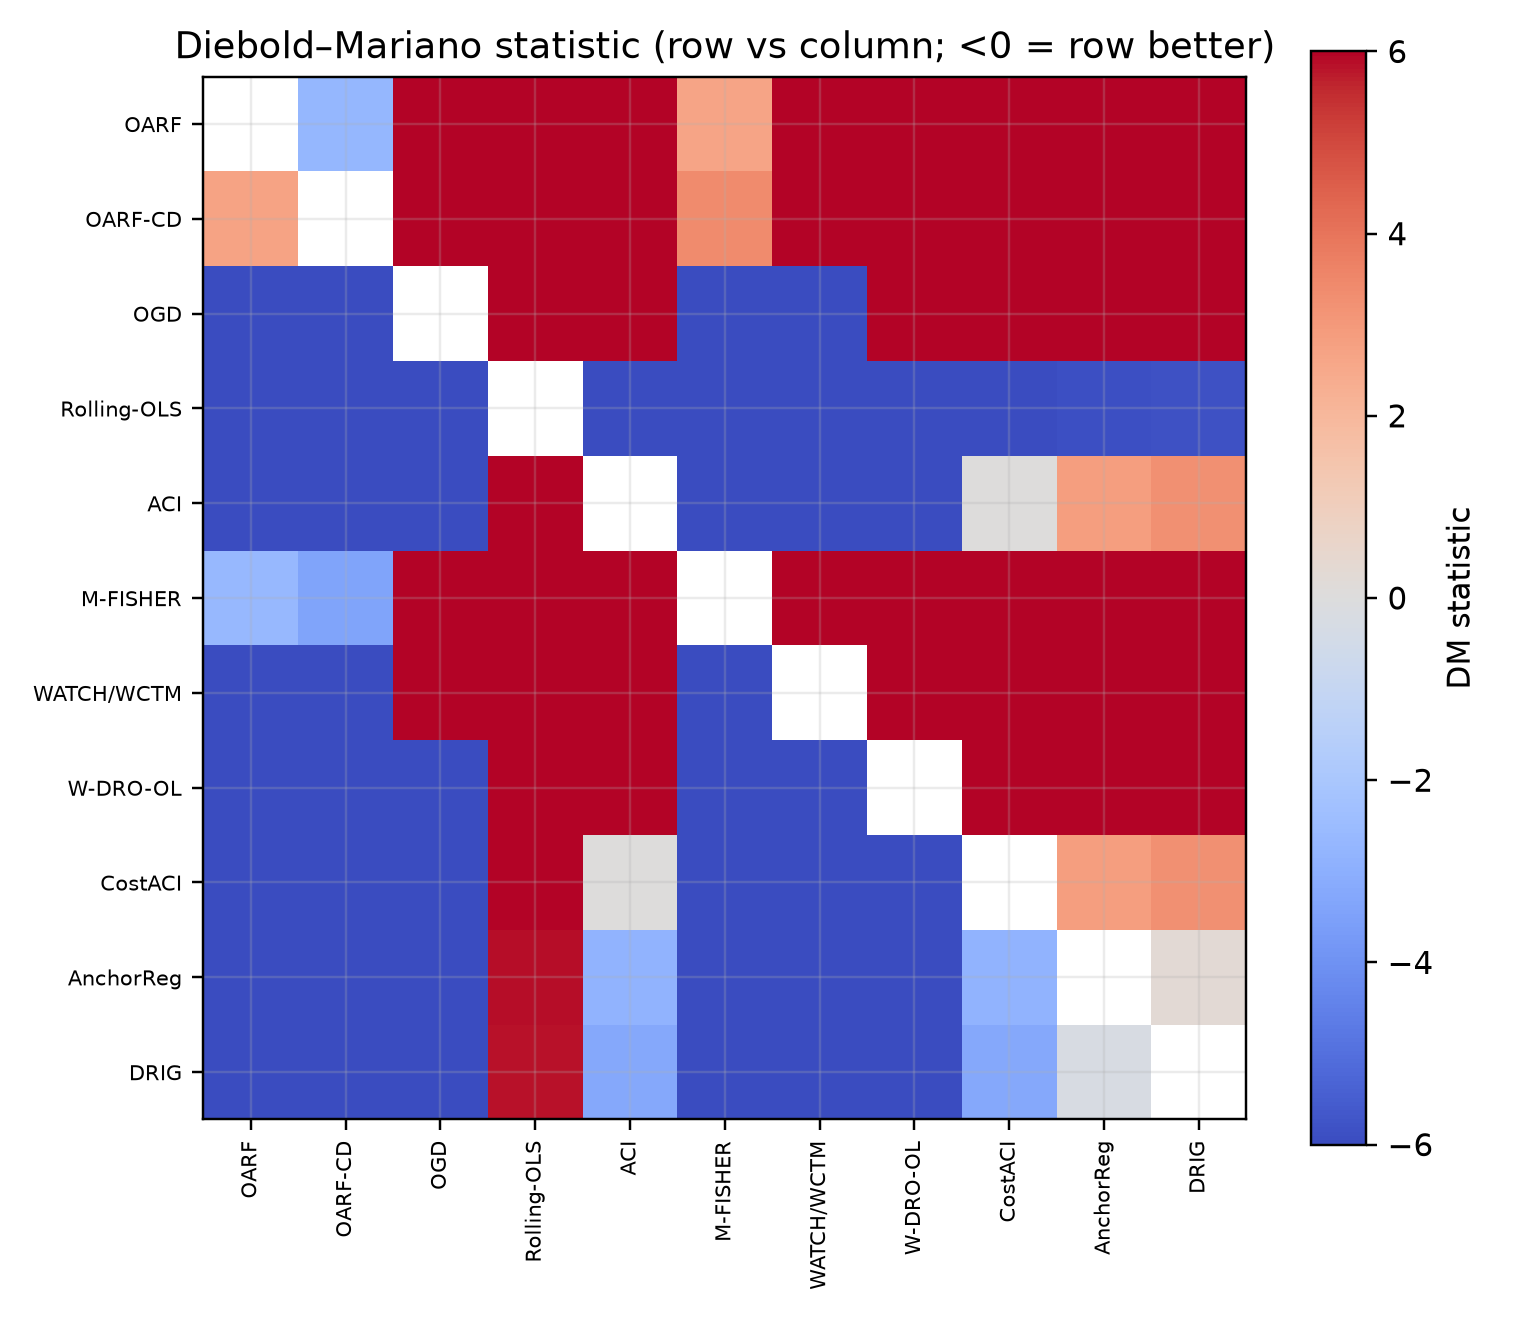
\includegraphics[width=0.66\textwidth]{fig8_dm_heatmap.png}
\caption{Pairwise Diebold--Mariano statistics on the synthetic benchmark (negative
= row significantly better than column).}
\label{fig:dm}
\end{figure}

\section{Discussion and limitations}\label{sec:discussion}
The evidence supports a precise claim. When regime shifts travel through an
observable channel with anchor-mediated confounding --- the structure economic
theory and the EU-ETS policy calendar suggest for energy and carbon markets ---
immunising the residual against that channel delivers large, near-oracle
interventional robustness fully online, at a small and tunable in-distribution
cost. When that structure is weak (efficient daily returns; mild realised-volatility
regimes), the method is competitive-to-better but not dominant, exactly as the
diluted-causal estimand of Remark~\ref{rem:honesty} predicts. We do not claim
causal identification, and the comparator is regime-conditional, not adversarial,
by necessity. The most important open item is a complete proof of step (iii) of
Theorem~\ref{thm:main} --- the concentration of the EMA cross-moments under
within-regime stationarity with a learned, slowly varying channel --- which would
extend the guarantee from the fixed-channel learner to \OARFCD{}. Other natural
extensions are a quantile/density head with interventional coverage guarantees and
a frictional-allocator head with decision-regret bounds.

\section{Conclusion}\label{sec:conclusion}
We introduced \OARF{}, a streaming anchor-robust forecaster that immunises against
economic regime shifts through the causal channel they travel, and a novel layer
that discovers that channel online. Against a target of interventional regret, the
fixed-channel learner enjoys an $O(\sqrt{T(1+K)})$ bound; empirically it halves-to-
quarters the worst-case interventional error of reactive and distributionally
robust competitors on a controlled benchmark and is never dominated on sixteen
years of energy-volatility data, with an interpretable, automatically discovered
channel. The message is that robustness should be spent where shifts actually
travel --- along the causal channel --- rather than over the agnostic balls of
distributionally robust optimisation.

\paragraph{Reproducibility.} All data-build scripts, the streaming
implementations of every method, the evaluation harness, and the figure code are
released; each table and figure in this paper is regenerated by
\texttt{run\_synthetic.py}, \texttt{run\_real.py} and \texttt{oarf/figures.py}.

\small
\bibliographystyle{plainnat}
\bibliography{references}

\end{document}
